\documentclass[12pt,a4paper]{article}
\usepackage[latin1]{inputenc}
\usepackage{amsmath}
\usepackage{amsfonts}
\usepackage{amssymb}
\usepackage{graphicx}

\graphicspath{{Figures/}}
\usepackage[margin=1in]{geometry}
\usepackage{graphicx}
\usepackage{rotating}
\usepackage{float}



\title{Co-clustering analysis of Covid-19 in the U.S.}
%\author{{\sc Gabriel Wallin}\\
		%{\small\texttt{gabriel.wallin@umu.se}}\vspace{0.1cm}\\	
%}\vspace{0.1cm}\vspace{0.1cm}

\usepackage[backend = biber, style=authoryear]{biblatex}
%\usepackage{biblatex}
\addbibresource{bibliography.bib}

\date{}
\begin{document}
\maketitle
\date	

\begin{abstract}
	\noindent In response to the global coronavirus pandemic, we study co-clustering of multivariate time-series data as a way to simultaneously cluster both geographical regions and time periods after the outbreak of the pandemic. The resulting blocks of clusters, identified with a latent block model component, are integrated with an extended SIR model that takes both geographical clusters as well as clusters of time periods into account. We consider US data (or global or both?) and show how the novel latent block SIR model produce better prediction accuracy of the epidemic, and gives further understanding of how the virus is spreading in different geographical regions during different periods of time. 
\end{abstract}	

\section{Introduction}

Following the advances of modern technology, it is nowadays not difficult to collect high frequency data. Smart phones, smart watches and similar devices for example makes it possible to gather a vast amount of data on each individual over time. With such data collected, it is of interest to summarize the data by homogeneous subgroups of the data matrix to, for example, increase individual prediction accuracy. Methods for clustering and classification of functional data has rapidly increased over time, and according to \cite{JacquesPreda}, there are four groups of clustering techniques for functional data: 1) the raw data methods that cluster the functions directly on the curves' finite set of point, 2) the filtering methods that first smooths the curves into basis functions and then clusters the basis expansion coefficients, 3) the adaptive methods that simultaneously cluster and express the functions in a finite dimensional space, and 4) the distance-based methods where classical algorithmic approaches such as k-means and hierarchical clustering are adapted to functional data. 

For all of the above clustering approaches there exist many studies considering univariate functional data $X(t)$. For multivariate functional data however, the number of studies are much fewer. Both \cite{Singhal} and \cite{Ieva} propose k-means clustering extended for multivariate functional data. This study however takes on a model-based approach to clustering using mixture models.  

The aim of this paper is to study the coronavirus pandemic, both on a global level and on a US level. A joint analysis of the number of cases and deaths is conducted in order to identify spatio-temporal clusters that captures the trend of the pandemic. We thus aim to cluster both the rows (the states) and the columns (the weeks) in the data matrix. In the statistical literature, this is known as co-clustering \cite{Bouveyron}. The analysis and theory presented assumes data in the form of multivariate functions, meaning that the data in itself are infinite dimensional. Some challenging problems for both theory and computation follows, which will be addressed as well. In the univariate case, each individual (i.e., country for this analysis) is described by a single function (stochastic process) 
$
X(t) \in \mathbb{R}
$, 
$
\forall t [0, T]
$,
whereas for the multivariate case 
$
\mathbf{X} = \mathbf{X}(t)_{t \in [0, T]}
$ 
where 
$
\mathbf{X}(t) = (X^1(t),\ldots, X^p(t))^\top
$.     

In a second stage of the analysis, the resulting blocks from the co-clustering of step one will be plugged into the well-known epidemiological SIR model. With information from the co-clusters, it is possible to make predictions about the pandemic for larger, homogeneous groups of countries. It is furthermore possible to enhance predictions by using the column clusters of time periods for which the pandemic spread in similar ways in the different row (country) clusters. Lastly, an important contribution of this study is the inclusion of dependence between observations in the recovery of the functional form of the data before the co-clustering is performed. 

QUESTION: How to formulate a model for wavelet smoothing in the case of peaked data?


\section{Functional Data Analysis}
We consider measurable, real-valued functions 
$
\mathbf{X}_1, \ldots, \mathbf{X}_n
$
that are realisations of a continuous, multivariate stochastic process 
$
\mathbf{X} = \{\mathbf{X}(t), \, t \in [0,T]\} = \{(X^1(t), \ldots, X^p(t))\}_{t \in [0, T]}
$
that belongs to the separable Hilbert space $L_2([0, 1], \mathbb{R})$ of square integrable functions on $[0, 1]$. The sample paths are denoted by 
$
\mathbf{X}_i = (X_i^1, \ldots, X_i^p) \in L_2(I), I=(0, T), 1 \leq i \leq n
$.

In many cases, the functions will only be observed at discrete time points on a fixed time grid, 
$
X^j(t_1), \ldots, X^j(t_s), 0 \leq t_1 \leq \ldots \leq t_s \leq 1 \, \forall 1 \leq i \leq n, 1 \leq j \leq p.
$
The first task thus becomes to recover the functional form from the discrete observations. With measurement errors often present in real data, smoothing techniques are often employed for this mean, assuming that the errors fluctuate around a smooth trajectory. A common approach is to make the assumption that the functions  
$
X_i^j(t) 
$
can be decomposed into a finite-dimensional space that is spanned by a set of basis functions. Denoting the basis functions of the $j$th component as 
$
(\phi_r^j(t))_{1\leq r \leq R_j}
$
and $R_j$ the number of basis functions, 
%
\begin{equation}\label{eq1}
X_i^j(t) = \sum_{r=1}^{R_j} c_{ir}^j(X_i^j) \phi_r^j(t)	
\end{equation}
%

Lastly, we gather the $c_{ir}^j$ coefficients and the $\phi_r^j$ basis functions in the matrices $\mathbf{C}$ and $\boldsymbol{\phi}$, where 

$$
\mathbf{C} = \begin{pmatrix}
	c_{11}^1 & \ldots & c_{1R_1}^1 & c_{11}^2 & \ldots & c_{1R_2}^2 & c_{11}^p & \ldots & c_{1R_p}^p \\
	\vdots & \vdots & \vdots & \vdots & \vdots & \vdots & \vdots & \vdots & \vdots \\ 
	c_{n1}^1 & \ldots & c_{nR_1}^1 & c_{n1}^2 & \ldots & c_{nR_2}^2 & c_{n1}^p & \ldots & c_{nR_p}^p
\end{pmatrix}
$$
and 

$$
\boldsymbol{\phi}(\mathbf{t}) = \begin{pmatrix}
	\phi_1^1(t) & \ldots & \phi_{R_1}^1(t) & 0 & \ldots & 0 & \ldots & 0 & \ldots & 0 \\
	0 & \ldots & 0 & \phi_1^2(t) & \ldots & \phi_{R_2}^2(t) & \ldots & 0 & \ldots & 0 \\ 
	\vdots & \vdots & \vdots & \vdots & \vdots & \vdots & \vdots & \vdots & \vdots & \vdots \\ 
	0 & \ldots & 0 & 0 & \ldots & 0 & \ldots & \phi_1^p(t) & \ldots & \phi_{R_p}^p(t)
\end{pmatrix}
$$
where the $r$th column equals the values of the $r$th basis function at time points $\mathbf{t}^\top = [t_1, t_2, \ldots, t_s]$.
With matrix notation, we can now express Equation (\ref{eq1}) as 

$$
\mathbf{X}(t) = \mathbf{C} \boldsymbol{\phi}^\top(t)
$$

Estimating the matrix $\mathbf{C}$ is often done using least squares \cite{ramsay2002functional}. Which basis to use, and how many basis functions to include is currently an open problem. It has however been recommended to use Fourier basis for data with a repetitive patterns, and a B-spline basis for most other cases \cite{schmutz2020clustering}. Regarding the number of basis functions to include has to be decided by the user as there are no clear rules on how to select it \cite{JacquesPreda}. 
 
\section{Functional Co-Clustering}

\subsection{Dependent Functional Data Analysis}
QUESTION: How to incorporate dependency between observations?

In functional data analysis, the second order structure of the functions are of central importance \cite{panaretos2013fourier}. For independent and identically distributed functional data, such structure is completely described by the covariance operator \cite{grenander1981abstract}. More recently, studies considering dependent functional data have emerged. 


\subsection{The Functional Latent Block Model}

The functional latent block model (FLBM, \cite{Bouveyron}) has been implemented to co-cluster the cases/deaths and the weeks. On a general level, the FLBM assumes the data matrix $\mathbf{x} = (\mathbf{x}_{ij})$, $i = 1,..., n$, $j = 1,..., p$, where each entry is a multivariate curve $\mathbf{x}_{ij} = (x_{ij}^1(t), \ldots, x_{ij}^S(t))$, $t \in [0, T]$ and where $s$ is the component of the multivariate curves. For the analyzed Covid-19 data, there are thus $n = 50$ states, $p = 12$ weeks and $s$ represents either cases or deaths. Since the functional form of the curves  $x_{ij}^s(t)$ is unknown, it is also assumed that the curves belong to a finite-dimensional space spanned by basis functions $\{\phi_r^s\}_{r=1, \dots, R_s}$ and that they can be expressed as linear combinations of those basis functions:
%
\begin{equation}
	x_{ij}^s(t) = \sum_{r=1}^{R_s} c^s_{ijr} \phi^s_r(t),
\end{equation}  
%
where $(c_{ijr}) = \mathbf{c}_{ij}$ denotes the basis expansion coefficients of each curve. The basis functions can for example be Fourier or spline bases, but it is yet unknown how to automatically select basis function and the number of basis functions \cite{Jacques}. The coefficients $c^s_{ijr}$ are often estimated using least squares smoothing \cite{Ramsay}.

The most common model for co-clustering is the latent block model (LBM, \cite{Govaert}). Let 
$
\mathbf{z} = (z_{ik})$, $j = 1,..., p
$,
$k = 1,..., K$ denote a binary random variable such that $z_{ik} = 1$ if individual $i$ belongs to row cluster $k$, and $\mathbf{w} = (w_{jl})$, $j = 1,..., p$, $l = 1,..., L$ denote a binary random variable such that $w_{jl} = 1$ if feature $j$ belongs to column cluster $l$. Co-clustering will yield subgroups, called blocks, such that $z_{ik} w_{jl} = 1$. It is assumed that $\mathbf{z}$ and $\mathbf{w}$ are independent from each other and that the random variables $\mathbf{x}$ are independent conditional on $\mathbf{z}$ and $\mathbf{w}$. 

From the independence assumption regarding $\mathbf{z}$ and $\mathbf{w}$, it follows that 
%
\begin{equation}\label{Distr. of c}
	p(c; \theta) = \sum_{z \in \mathbf{Z}} \sum_{w \in \mathbf{W}} p(z; \theta) p(w; \theta) p(c|z, w; \theta)
\end{equation}  
% 
where $c = (c_{ij})_{ij}$. Now let $\alpha_k \in [0,1]$ and $\beta_l \in [0,1]$ denote the respective row and column mixing proportions such that they both sum to 1 and 
$
p(z; \theta) = \prod_{ik} \alpha_k^{z_{ik}} 
$
and 
$
p(w; \theta) = \prod_{ik} \beta_l^{w_{jl}}. 
$
If it further is assumed that the $c_{ij}$ basis expansion coefficients are independent and generated by a distribution that is block-specific,
$
p(c|z, w; \theta) = \prod_{ijkl} p(c_{ij}; \theta_{kl})^{z_{ik} w_{jl}},
$
the distribution in (\ref{Distr. of c}) can be expressed as
%
\begin{equation}
	p(c; \theta) = \sum_{z \in \mathbf{Z}} \sum_{w \in \mathbf{W}} \prod_{ik} \alpha_k^{z_{ik}} \prod_{ik} \beta_l^{w_{jl}} \prod_{ijkl} p(c_{ij}; \theta_{kl})^{z_{ik} w_{jl}}.
\end{equation}

\section{Estimation}
Using the LBM to cluster the rows and columns implies a data structure with missing values on two variables, $z$ and $w$. It therefore follows that the commonly used EM algorithm does not work since there will be too many terms to compute in the E-step. This study therefore implements the estimation technique suggested in \cite{Bouveyron} by using a stochastic version of the EM-algorithm and embedding a Gibbs sampler that generates $z$ and $w$. In this way it is possible to circumvent having to compute their joint probability distribution. Since the algorithm needs initial values for the column partitions and the parameters, k-means clustering is used to initialize the row and column partitions. From these partitions it is possible to deduce the initial parameter values. Lastly, the number of row and column clusters are chosen by maximizing the Integrated Classification Likelihood (ICL) value, see \cite{Bouveyron} for the details.

\section{Data}
In Table 1, the data is summarized, together with information about when the first Covid-19 case was registered at each state. This date differs a lot between states; for example, in Alabama, the first case was reported at the 13th of March, wheras the first case in California was reported at the 25th of January. The first case in the country was reported in Washington at the 21st of January, however most states had their first reported case in early March. For all states, there are no "missing values" after the date of a first registered case, meaning there are confirmed cases each day for every state starting from the first day of case registration. 

In Table 1, there is also a column with the number of deaths per case. This information is also contained in Figure 1, where the number of deaths in relation to state population size is plotted against the number of deaths in relation to the number of cases. The mortality of the virus for the different states appears a bit different compared to only looking at death numbers relative to state population size. For states with a low fraction of deaths relative to state population size, the mortality for confirmed cases is much higher compared to the states with a relatively larger fraction of deaths.

Figure 2 and 3 show the trajectories of deaths and cases over the whole period, starting from the first registered case in January. The trajectories show each state, with color indicating which row cluster it belongs to. Figure 4 shows the five row clusters as different panels. 

In Figure 5, the total number of cases are given for each state. As is apparent, the state of New York has almost 4 000 000 infected people, compared to the state average of 222 115 people. 

In Figure 6, the total number of deaths are displayed for each state. The state average equals 8410.3 deaths. 


\begin{table}[H]
	\centering
	\resizebox{\columnwidth}{!}{%
	\begin{tabular}{rllrrrrrl}
		\hline
		& State & Abbr. & Cases & Deaths & Deaths of cases & Fraction cases & Fraction deaths & First case \\ 
		\hline
		1 & Alabama & AL & 559482 & 20475 & 0.04 & 0.11 & 0.00 & 2020-03-13 \\ 
		2 & Alaska & AK & 22826 & 447 & 0.02 & 0.03 & 0.00 & 2020-03-12 \\ 
		3 & Arizona & AZ & 616257 & 27696 & 0.04 & 0.08 & 0.00 & 2020-01-26 \\ 
		4 & Arkansas & AR & 230964 & 4591 & 0.02 & 0.08 & 0.00 & 2020-03-11 \\ 
		5 & California & CA & 3751385 & 143726 & 0.04 & 0.09 & 0.00 & 2020-01-25 \\ 
		6 & Colorado & CO & 1023645 & 52079 & 0.05 & 0.18 & 0.01 & 2020-03-05 \\ 
		7 & Connecticut & CT & 1734813 & 142974 & 0.08 & 0.49 & 0.04 & 2020-03-08 \\ 
		8 & Delaware & DE & 327783 & 11368 & 0.03 & 0.34 & 0.01 & 2020-03-11 \\ 
		9 & Florida & FL & 2275776 & 87198 & 0.04 & 0.11 & 0.00 & 2020-03-01 \\ 
		10 & Georgia & GA & 1723453 & 73906 & 0.04 & 0.16 & 0.01 & 2020-03-02 \\ 
		11 & Hawaii & HI & 37820 & 851 & 0.02 & 0.03 & 0.00 & 2020-03-06 \\ 
		12 & Idaho & ID & 132183 & 3647 & 0.03 & 0.07 & 0.00 & 2020-03-13 \\ 
		13 & Illinois & IL & 4026956 & 175007 & 0.04 & 0.32 & 0.01 & 2020-01-24 \\ 
		14 & Indiana & IN & 1268191 & 75820 & 0.06 & 0.19 & 0.01 & 2020-03-06 \\ 
		15 & Iowa & IA & 587883 & 14438 & 0.02 & 0.19 & 0.00 & 2020-03-08 \\ 
		16 & Kansas & KS & 329552 & 8648 & 0.03 & 0.11 & 0.00 & 2020-03-07 \\ 
		17 & Kentucky & KY & 343811 & 16175 & 0.05 & 0.08 & 0.00 & 2020-03-06 \\ 
		18 & Louisiana & LA & 1838336 & 118310 & 0.06 & 0.40 & 0.03 & 2020-03-09 \\ 
		19 & Maine & ME & 83770 & 3314 & 0.04 & 0.06 & 0.00 & 2020-03-12 \\ 
		20 & Maryland & MD & 1691454 & 80878 & 0.05 & 0.28 & 0.01 & 2020-03-05 \\ 
		21 & Massachusetts & MA & 3898291 & 235391 & 0.06 & 0.57 & 0.03 & 2020-02-01 \\ 
		22 & Michigan & MI & 2591288 & 226105 & 0.09 & 0.26 & 0.02 & 2020-03-10 \\ 
		23 & Minnesota & MN & 615792 & 28982 & 0.05 & 0.11 & 0.01 & 2020-03-06 \\ 
		24 & Mississippi & MS & 507678 & 22152 & 0.04 & 0.17 & 0.01 & 2020-03-11 \\ 
		25 & Missouri & MO & 526853 & 25426 & 0.05 & 0.09 & 0.00 & 2020-03-07 \\ 
		26 & Montana & MT & 28879 & 845 & 0.03 & 0.03 & 0.00 & 2020-03-13 \\ 
		27 & Nebraska & NE & 396122 & 5279 & 0.01 & 0.20 & 0.00 & 2020-02-17 \\ 
		28 & Nevada & NV & 344223 & 16099 & 0.05 & 0.11 & 0.01 & 2020-03-05 \\ 
		29 & New Hampshire & NH & 162265 & 6877 & 0.04 & 0.12 & 0.01 & 2020-03-02 \\ 
		30 & New Jersey & NJ & 7234185 & 448178 & 0.06 & 0.81 & 0.05 & 2020-03-04 \\ 
		31 & New Mexico & NM & 253369 & 10331 & 0.04 & 0.12 & 0.00 & 2020-03-11 \\ 
		32 & New York & NY & 18775939 & 1376727 & 0.07 & 0.97 & 0.07 & 2020-03-01 \\ 
		33 & North Carolina & NC & 840922 & 28059 & 0.03 & 0.08 & 0.00 & 2020-03-03 \\ 
		34 & North Dakota & ND & 81356 & 1836 & 0.02 & 0.11 & 0.00 & 2020-03-11 \\ 
		35 & Ohio & OH & 1255910 & 69208 & 0.06 & 0.11 & 0.01 & 2020-03-09 \\ 
		36 & Oklahoma & OK & 251520 & 13684 & 0.05 & 0.06 & 0.00 & 2020-03-06 \\ 
		37 & Oregon & OR & 176614 & 6589 & 0.04 & 0.04 & 0.00 & 2020-02-28 \\ 
		38 & Pennsylvania & PA & 3072958 & 181844 & 0.06 & 0.24 & 0.01 & 2020-03-06 \\ 
		39 & Rhode Island & RI & 548757 & 21141 & 0.04 & 0.52 & 0.02 & 2020-03-01 \\ 
		40 & South Carolina & SC & 426778 & 16664 & 0.04 & 0.08 & 0.00 & 2020-03-06 \\ 
		41 & South Dakota & SD & 171116 & 1698 & 0.01 & 0.19 & 0.00 & 2020-03-10 \\ 
		42 & Tennessee & TN & 808879 & 13773 & 0.02 & 0.12 & 0.00 & 2020-03-05 \\ 
		43 & Texas & TX & 2181099 & 57768 & 0.03 & 0.08 & 0.00 & 2020-02-12 \\ 
		44 & Utah & UT & 340148 & 3557 & 0.01 & 0.11 & 0.00 & 2020-02-25 \\ 
		45 & Vermont & VT & 54998 & 2867 & 0.05 & 0.09 & 0.00 & 2020-03-07 \\ 
		46 & Virginia & VA & 1294819 & 42147 & 0.03 & 0.15 & 0.00 & 2020-03-07 \\ 
		47 & Washington & WA & 1030357 & 53549 & 0.05 & 0.14 & 0.01 & 2020-01-21 \\ 
		48 & West Virginia & WV & 75760 & 2701 & 0.04 & 0.04 & 0.00 & 2020-03-17 \\ 
		49 & Wisconsin & WI & 570738 & 21283 & 0.04 & 0.10 & 0.00 & 2020-02-05 \\ 
		50 & Wyoming & WY & 37265 & 433 & 0.01 & 0.06 & 0.00 & 2020-03-11 \\ 
		\hline
	\end{tabular}
    }
\caption{The number of cases, deaths and fraction of Covid-19 cases per state together with the date of the first reported Covid-19 case.}
\end{table}
 



\begin{figure}[H]
	\begin{center}
	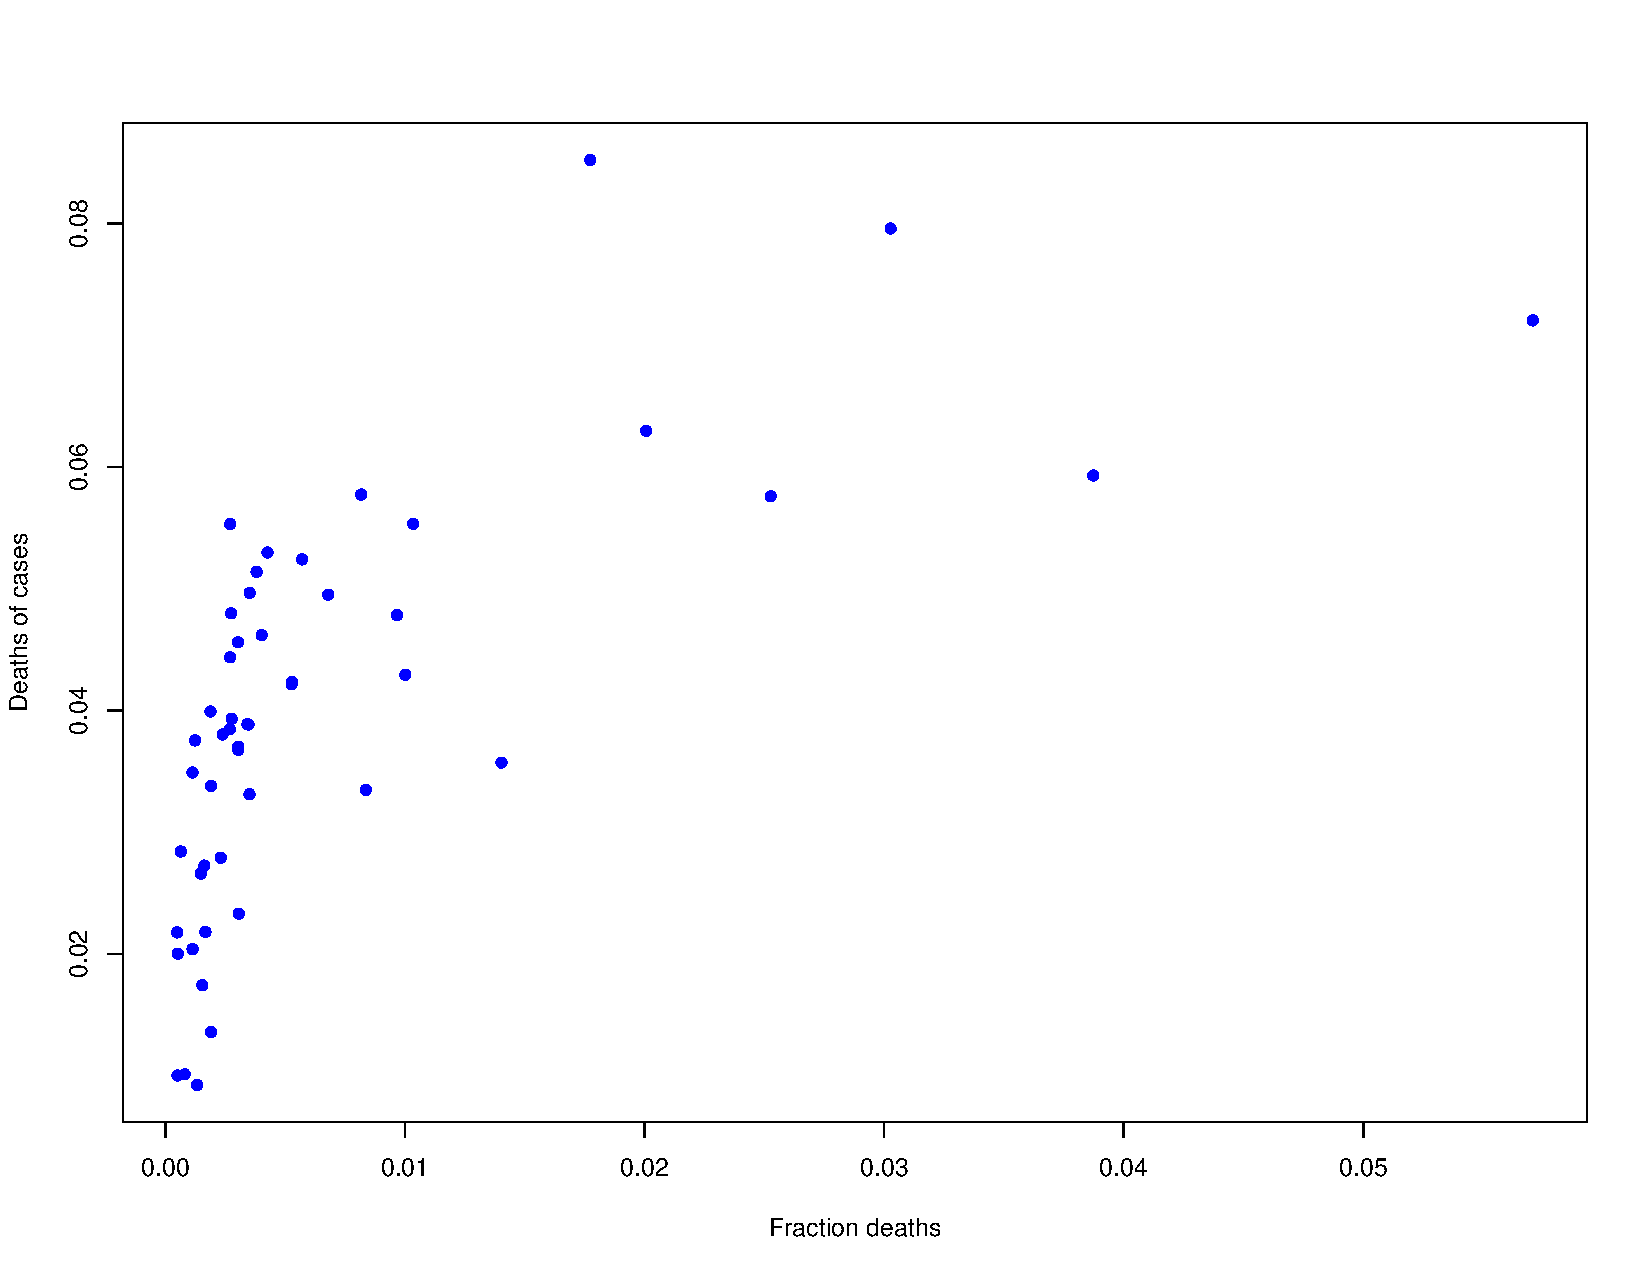
\includegraphics[width=\columnwidth]{rplot.pdf}
	\caption{Fraction of deaths plotted against fraction of cases.}
	\label{Fig1}
	\end{center}
\end{figure}


\begin{figure}[H]
	\begin{center}
		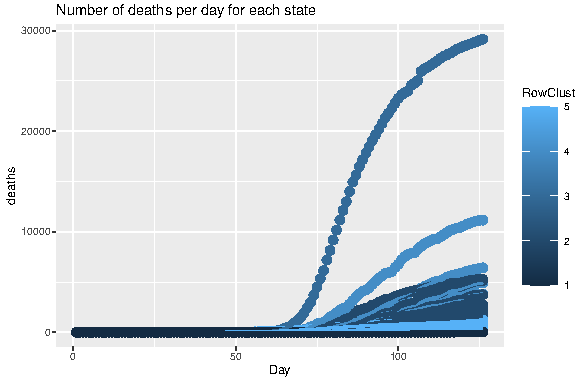
\includegraphics{Trajectories_deaths.pdf}
		\caption{Trajectories of deaths per day for each state.}
		\label{fig14}
	\end{center}
\end{figure}


\begin{figure}[H]
	\begin{center}
		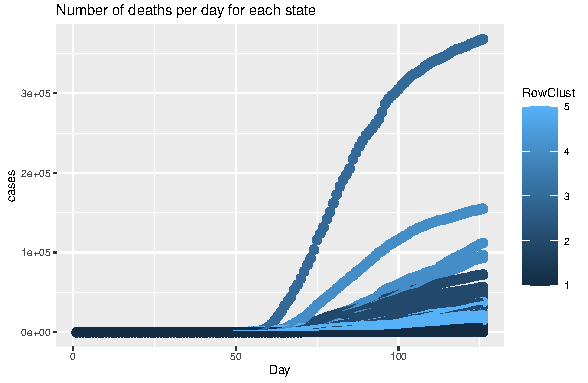
\includegraphics{Trajectories_cases.pdf}
		\caption{Trajectories of deaths per day for each state.}
		\label{fig15}
	\end{center}
\end{figure}

\begin{figure}[H]
	\begin{center}
		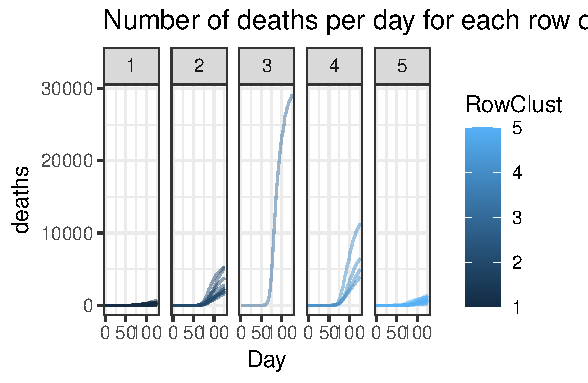
\includegraphics{TrajectoriesPerCluster_deaths.pdf}
		\caption{Trajectories of deaths per day for each row cluster.}
		\label{fig16}
	\end{center}
\end{figure}

 In Figure 5 and 6 the number of cases and deaths per state are displayed. It is clear that the state of New York and state of New Jersey stand out. 

\begin{sidewaysfigure}[ht]
	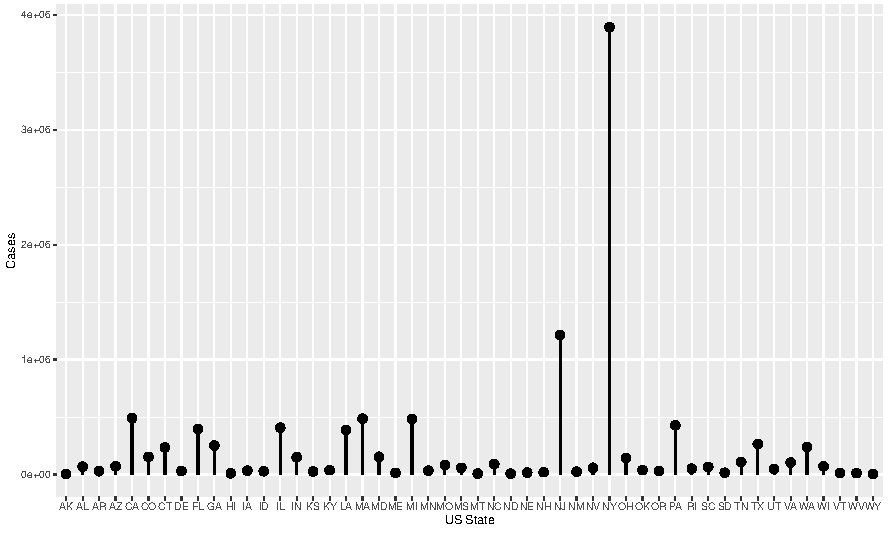
\includegraphics[width=\columnwidth]{NumberOfCases.pdf}
	\label{fig4}
	\caption{The number of Covid-19 cases per state.}
\end{sidewaysfigure}

\begin{sidewaysfigure}[ht]
	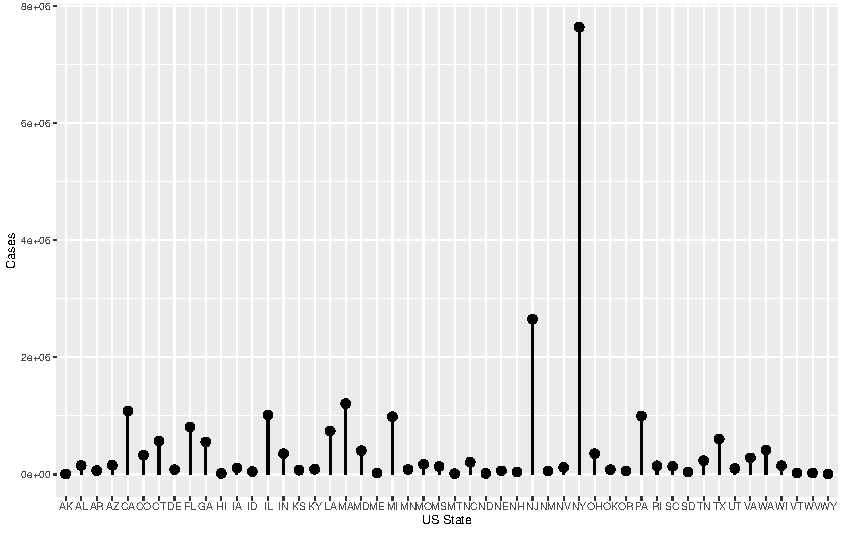
\includegraphics[width=\columnwidth]{NumberOfDeaths.pdf}
	\label{fig5}
	\caption{The number of Covid-19 deaths per state.}
\end{sidewaysfigure}

\section{Co-Clustering Results}

\subsection{Univariate co-clustering of Covid-19 cases}
In Figure 7 the block mean functions for the variable "Cases" is shown. For the row clusters 1 and 5, there are no period variations. For row cluster three there are on the otherside distinct differences for the different column clusters.

In Figure 8 the column clusters are displayed over the measurement period. There is a clear division between the clusters, with March being almost entirely represented by column cluster 1 and May by column cluster 5. In April, clusters 2 and 3 are representing half of the month each. There thus seem to be distinct periods in the virus outbreak, where the spread of the virus continuously enters new phases along with time. 

%
%% CASES
%
\begin{figure}[H]
	\begin{center}
		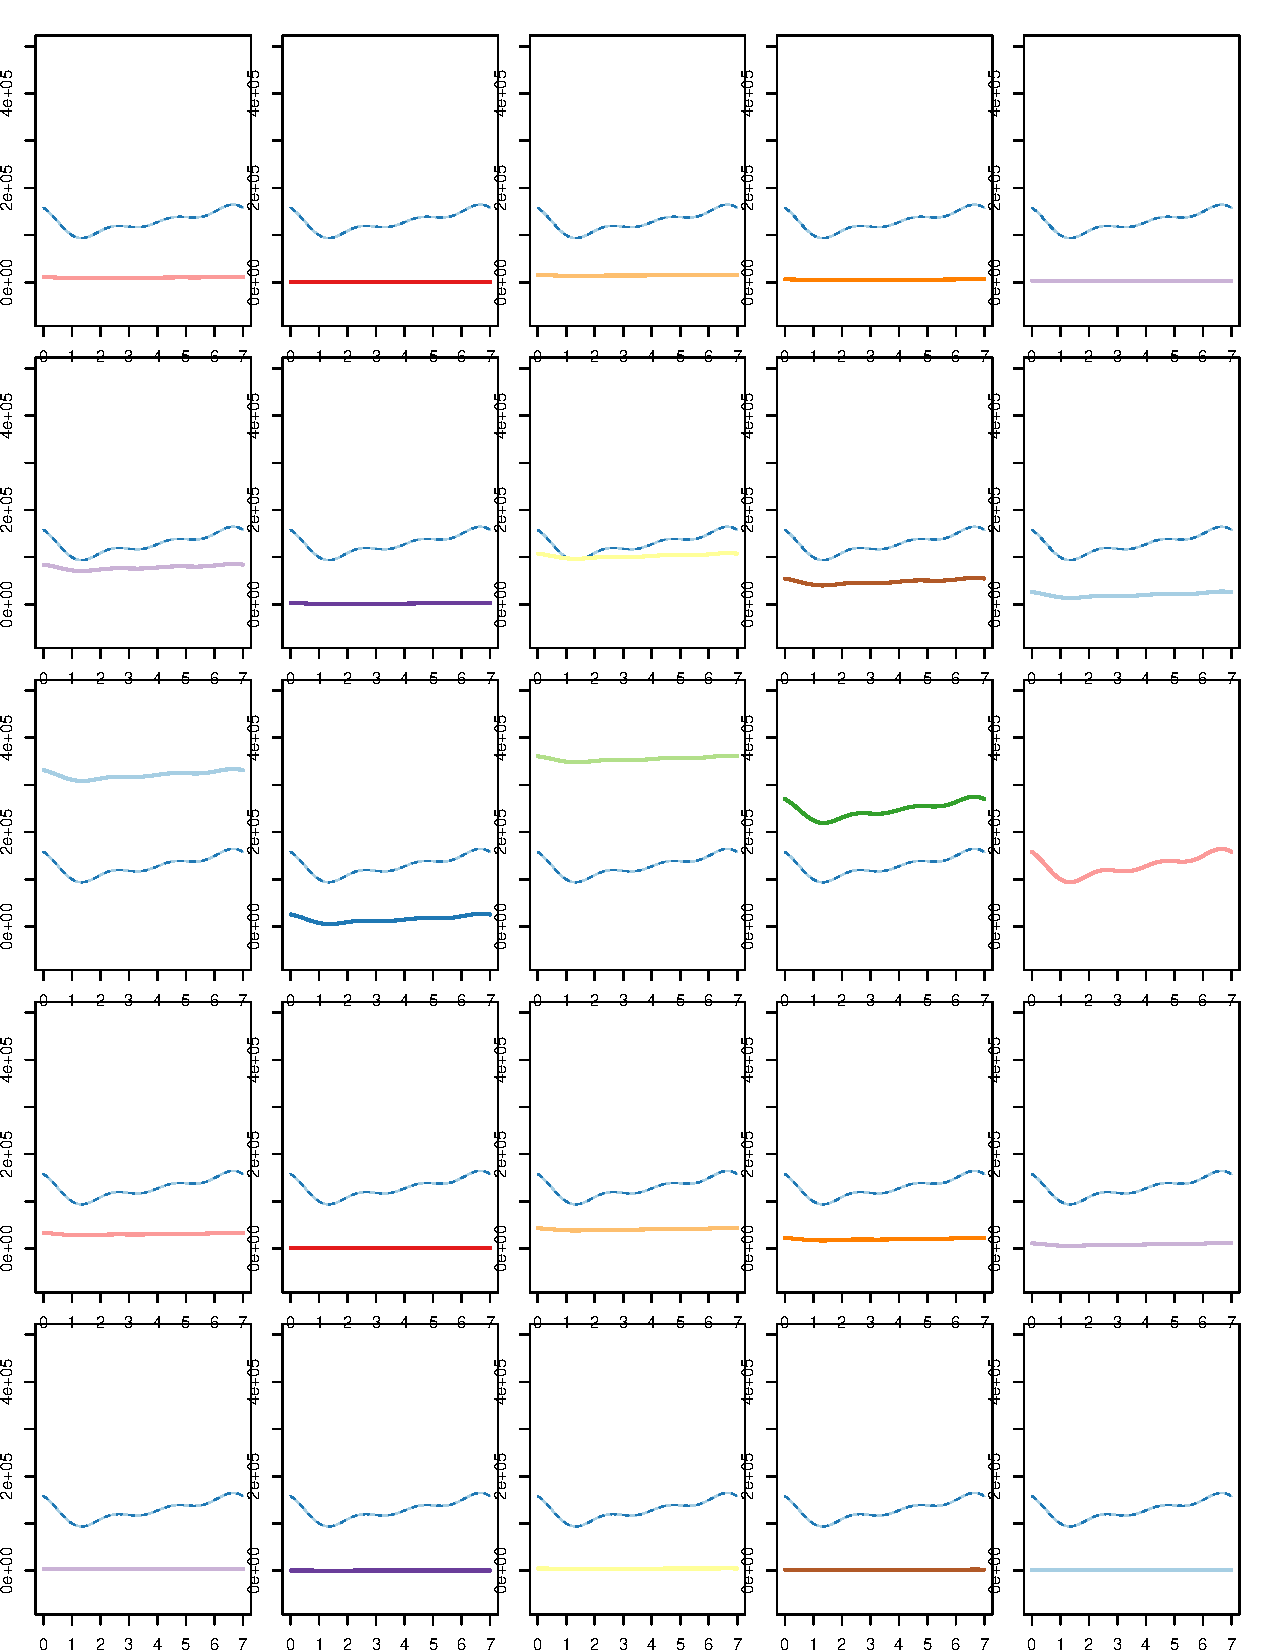
\includegraphics[width=\columnwidth]{Cases_blocks.pdf}
		\caption{Blocks showing the mean functions for the univariate co-clustering of Covid-19 cases.}
		\label{fig6}
	\end{center}
\end{figure}

\begin{figure}[H]
	\begin{center}
		\includegraphics[width=\columnwidth]{Cases_calendar.pdf}
		\caption{Calendar showing the column clusters for the univariate co-clustering of Covid-19 cases.}
		
	\end{center}
\end{figure}

\begin{figure}[H]
	\begin{center}
		\includegraphics[width=\columnwidth]{Cases_map.pdf}
		\caption{A map of the american states showing the row clusters.}
		
	\end{center}
\end{figure}

\begin{figure}[H]
	\begin{center}
		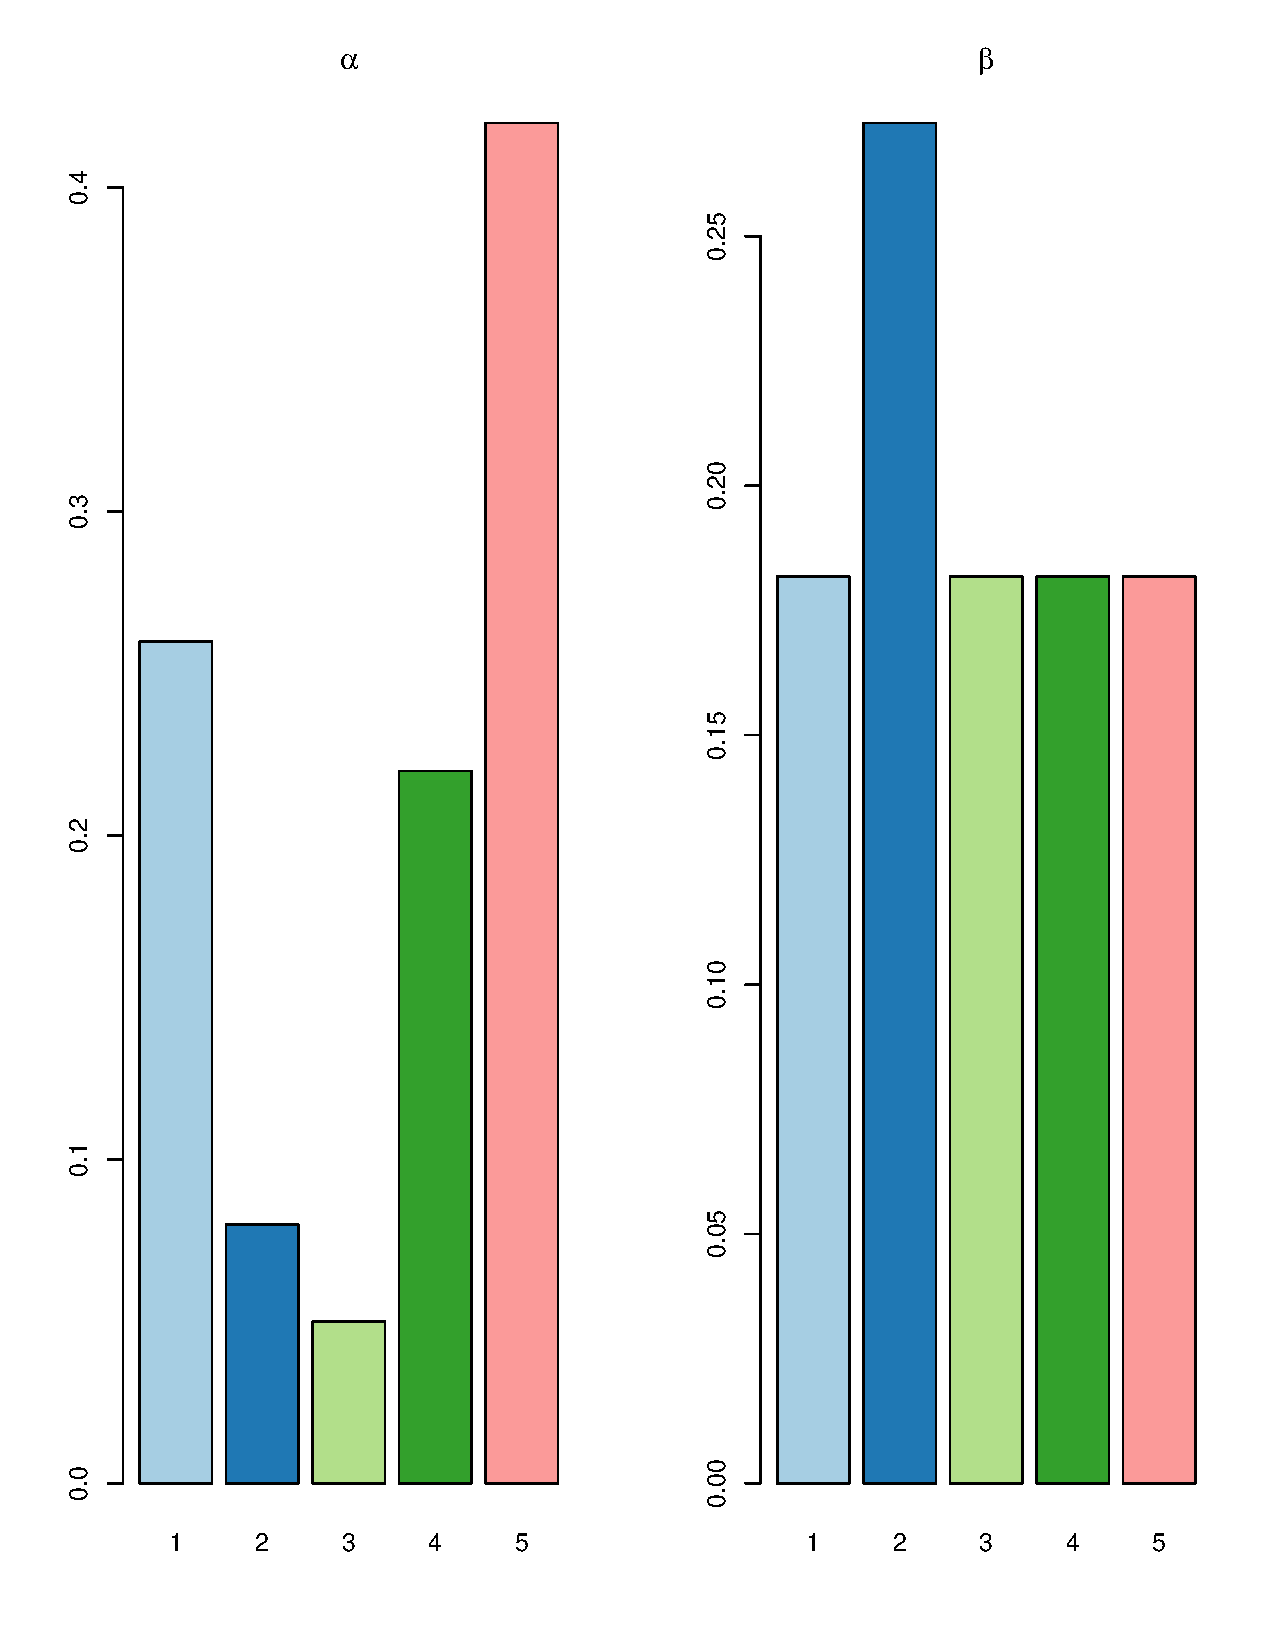
\includegraphics[width=\columnwidth]{Cases_prop.pdf}
		\caption{The proportions of states and weeks belonging to the row and column clusters, respectively.}
		
	\end{center}
\end{figure}
%
%% DEATHS
%

\subsection{Univariate co-clustering of Covid-19 deaths}
\begin{figure}[H]
	\begin{center}
		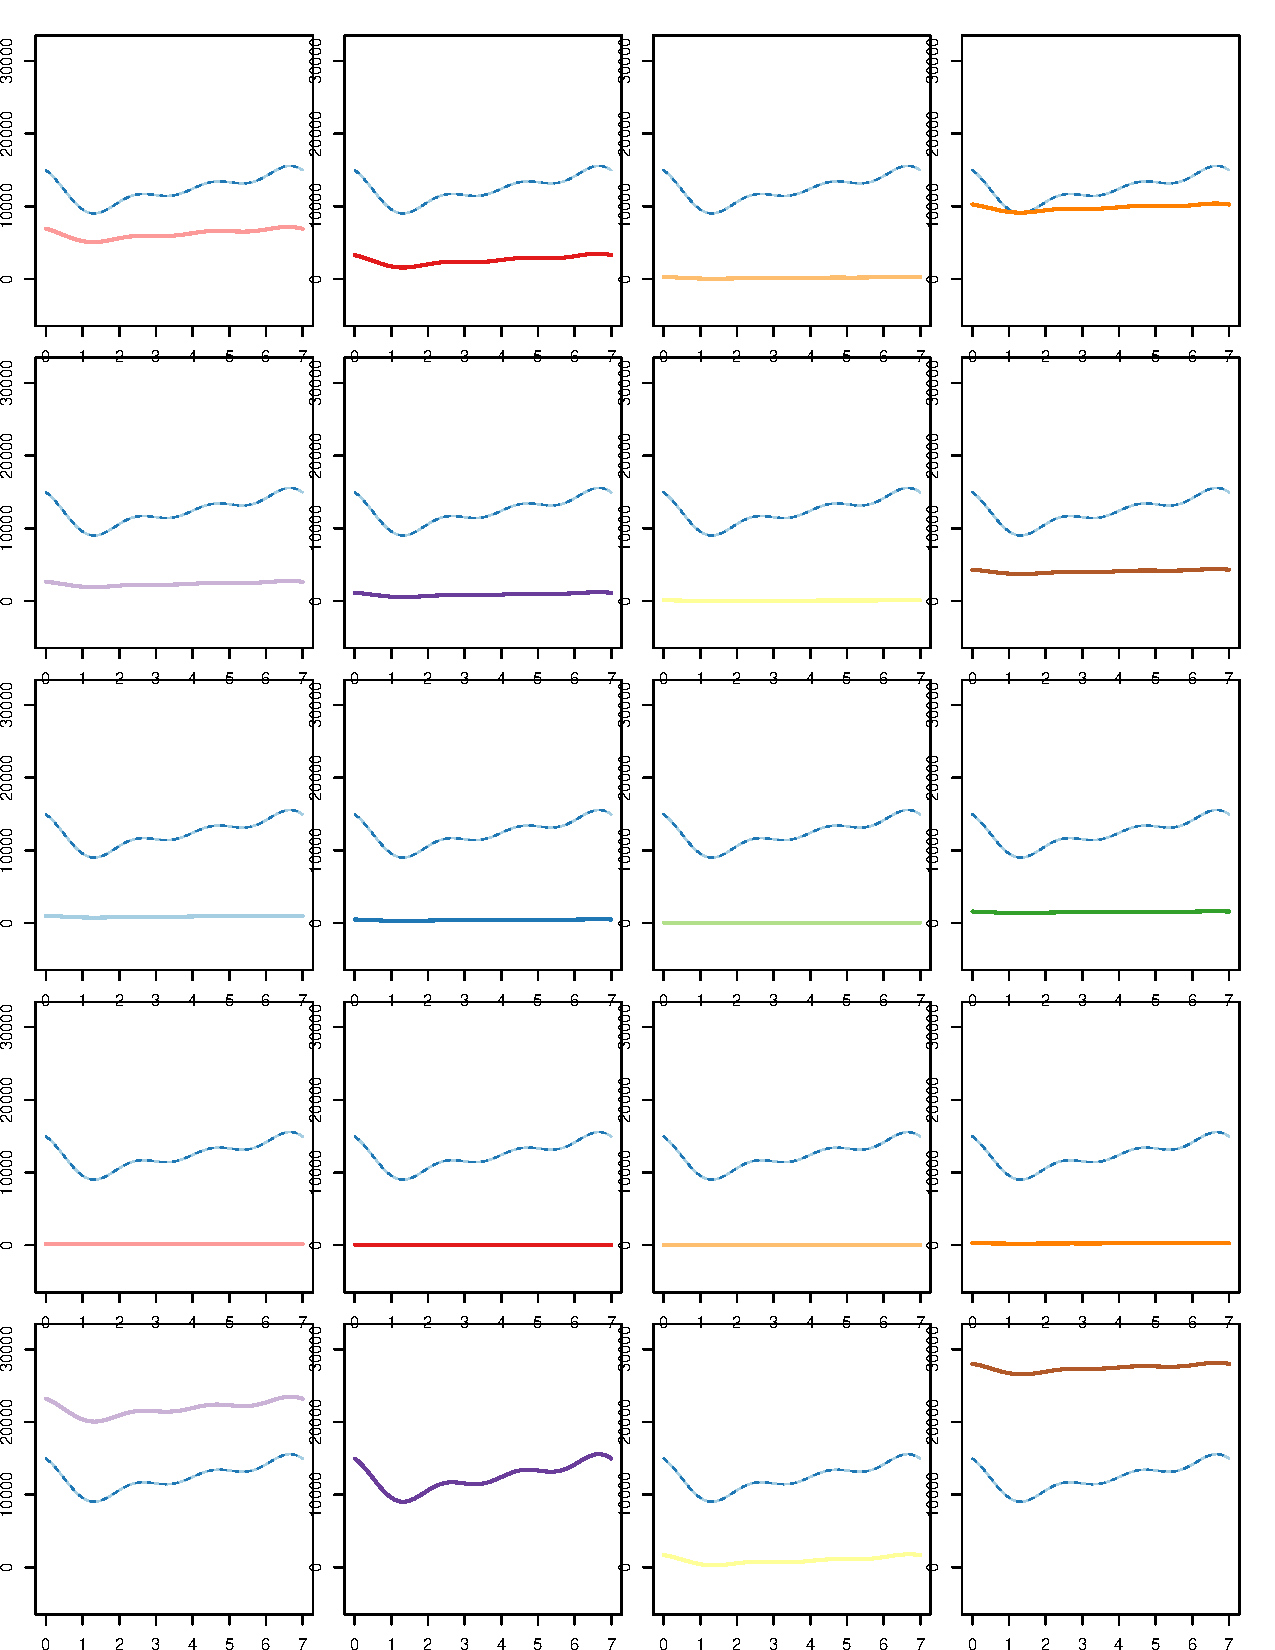
\includegraphics[width=\columnwidth]{Deaths_blocks.pdf}
		\caption{Blocks showing the mean functions for the univariate co-clustering of Covid-19 cases.}
		\label{fig6}
	\end{center}
\end{figure}

\begin{figure}[H]
	\begin{center}
		\includegraphics[width=\columnwidth]{Deaths_calendar.pdf}
		\caption{Calendar showing the column clusters for the univariate co-clustering of Covid-19 cases.}
		
	\end{center}
\end{figure}

\begin{figure}[H]
	\begin{center}
		\includegraphics[width=\columnwidth]{Deaths_map.pdf}
		\caption{A map of the american states showing the row clusters.}
		
	\end{center}
\end{figure}

\begin{figure}[H]
	\begin{center}
		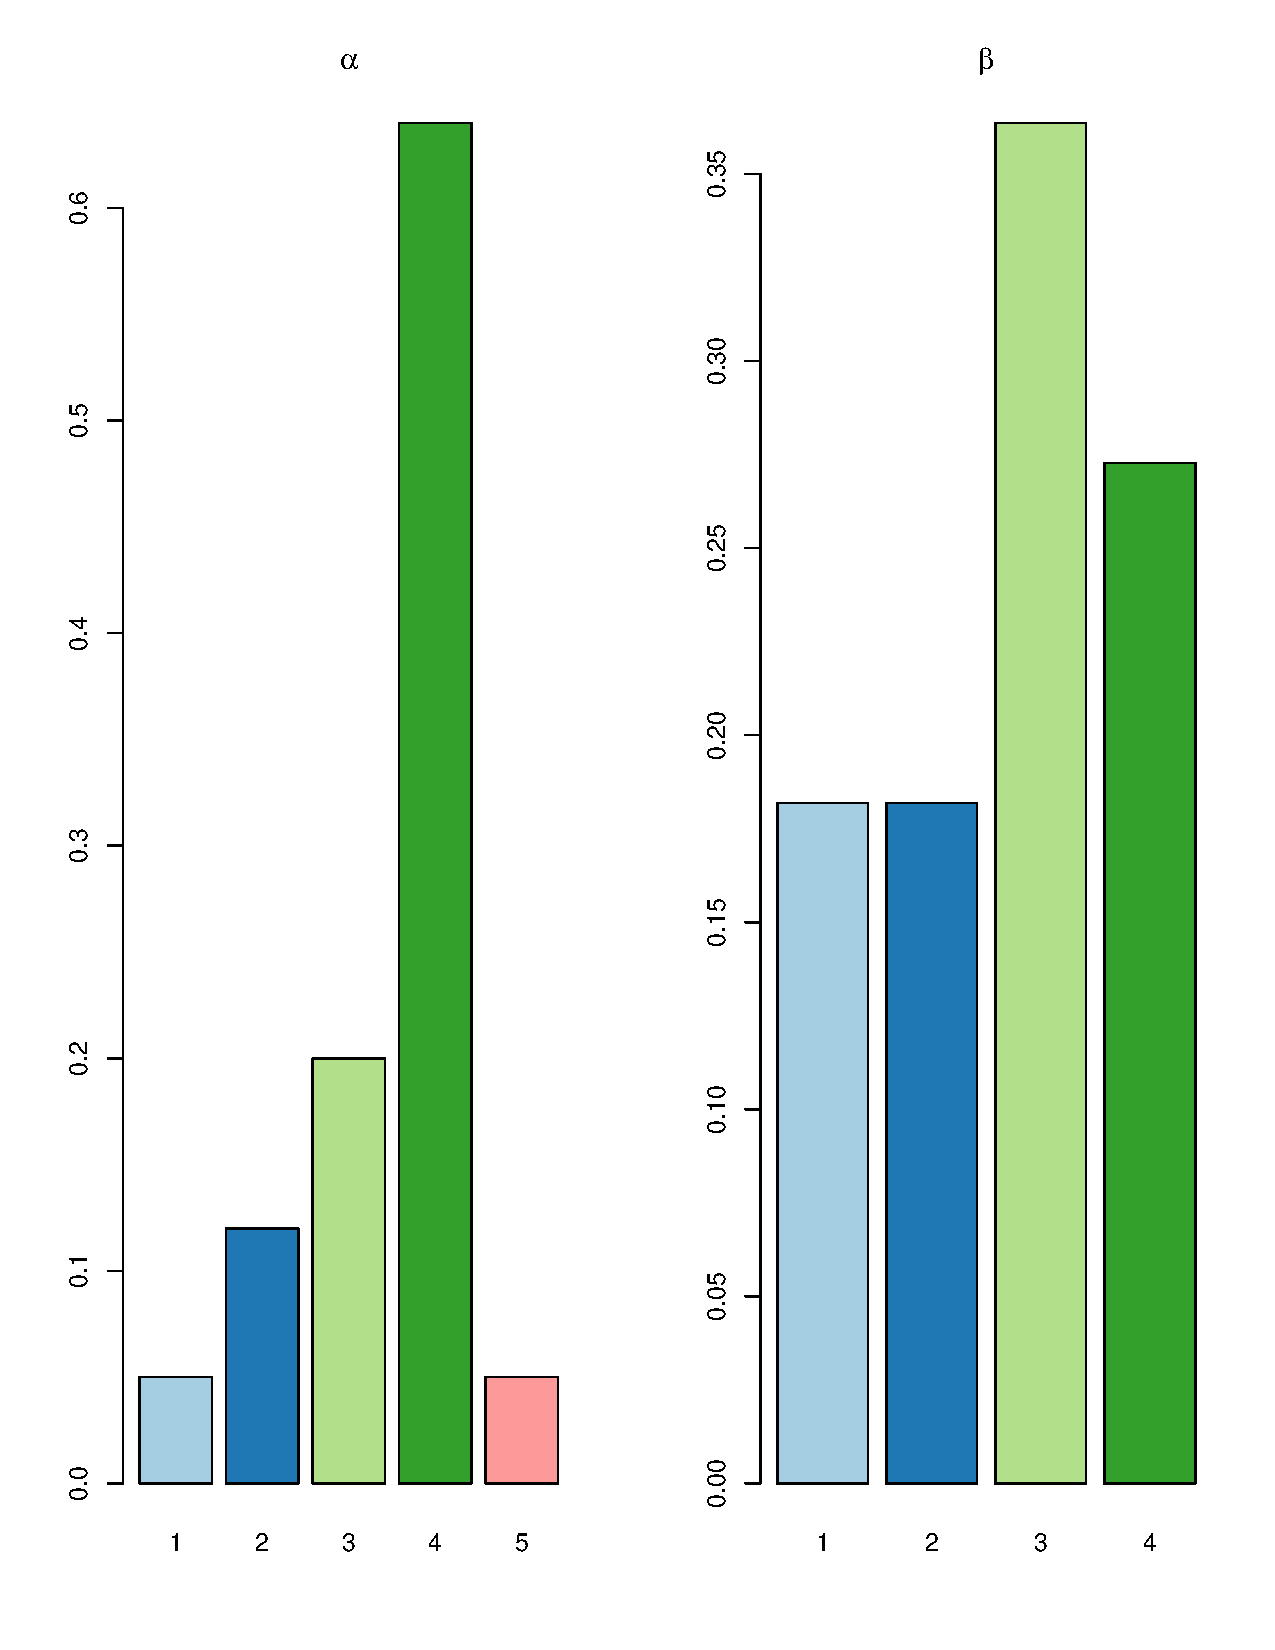
\includegraphics[width=\columnwidth]{Deaths_prop.pdf}
		\caption{The proportions of states and weeks belonging to the row and column clusters, respectively.}
		
	\end{center}
\end{figure}

In the next step, a multivariate function considering both deaths and cases is adopted.
%
%% Multivariate
%
\subsection{Multivariate co-clustering of Covid-19 cases and deaths}
\begin{figure}[H]
	\begin{center}
		\includegraphics[width=\columnwidth]{Multi_calendar.pdf}
		\caption{Calendar showing the column clusters for the multivariate co-clustering of Covid-19 cases and deaths.}
		
	\end{center}
\end{figure}

\begin{figure}[H]
	\begin{center}
		\includegraphics[width=\columnwidth]{Multi_map.pdf}
		\caption{A map of the american states showing the row clusters.}
		
	\end{center}
\end{figure}

\begin{figure}[H]
	\begin{center}
		\includegraphics[width=\columnwidth]{Multi_prop.pdf}
		\caption{The proportions of states and weeks belonging to the row and column clusters, respectively.}
		
	\end{center}
\end{figure} 

\section{Epidemiology Model for Prediction}
SIR model.

\section{Current problems}
Need to fix the block plots, scale the figures and comment them. Need to produce block plot for multivariate case. Need to figure out how the prediction step should look like. How does the SIR model work? What can be done? What has been done in previous studies? Is it possible to incorporate other information to make better predictions? What kind of information is available?
\printbibliography

\end{document}

